

 \documentclass[onecolumn, letterpaper]{igs}

% but use this version when submitting your article:
% \documentclass[review,oneside, letterpaper]{igs}

  \usepackage{igsnatbib}
  \usepackage{lmodern}
\usepackage{amsmath,amssymb,amsthm}
\usepackage{wrapfig}
\usepackage{enumitem}
\usepackage{multirow}
\usepackage{tabularx}
\usepackage{booktabs}
\usepackage{lscape}
\usepackage{threeparttable}
\usepackage{dblfloatfix}
\usepackage[pdftex]{graphicx}
 \usepackage{epstopdf}
\usepackage{caption}

\newcolumntype{C}{>{\centering\arraybackslash}X}
\renewcommand{\tabularxcolumn}[1]{m{#1}}%

 
\setcounter{table}{0}
\renewcommand{\thetable}{S\arabic{table}}

\setcounter{figure}{0}
\renewcommand{\thefigure}{S\arabic{figure}}
  
\begin{document}

\section*{Supplementary material}

\subsection*{Topographic parameters}

%% TOPOGRAPHIC PARAMETERS EXPLAINED

Topographic parameters are easy-to-calculate proxies for physical processes, such as orographic precipitation, solar radiation effects, wind redistribution and preferential deposition. We derive all parameters (Table \ref{tab:TopoParams}) for our study from a SPOT-5 DEM ($40\times40$ m) \citep{Korona2009}. Two DEMs are stitched together to cover the Donjek Range. An iterative 3D-coregistration algorithm \citep{Berthier2007} is used to correct the horizontal ($\sim$2\,m E, $\sim$4\,m N) and vertical (5.4\,m) discrepancy between the two DEMs before stitching. 

Visual inspection of the curvature fields calculated using the full DEM shows a noisy spatial distribution. To find an appropriate scale at which the relevant curvature is calculated, various smoothing algorithms and sizes are applied and the combination that produces the highest correlation between curvature and gridcell-averaged WB is chosen. Inverse-distance weighted, Gaussian and gridcell-average smoothing methods, all with window sizes of 3$\times$3, 5$\times$5, 7$\times$7 and 9$\times$9 gridcells are used. Gridcell-average smoothing with a 7$\times$7 window resulted in the highest overall correlation between curvature (second derivative) and gridcell-averaged WB as well as slope (first derivative) and gridcell-averaged WB. We use the smoothed DEM to calculate curvature ($\kappa$), slope ($m$), aspect ($\alpha$) and ``northness'' ($N$).


%% TOPO SAMPLED VS FULL
\begin{figure*}[b]
	\centering
	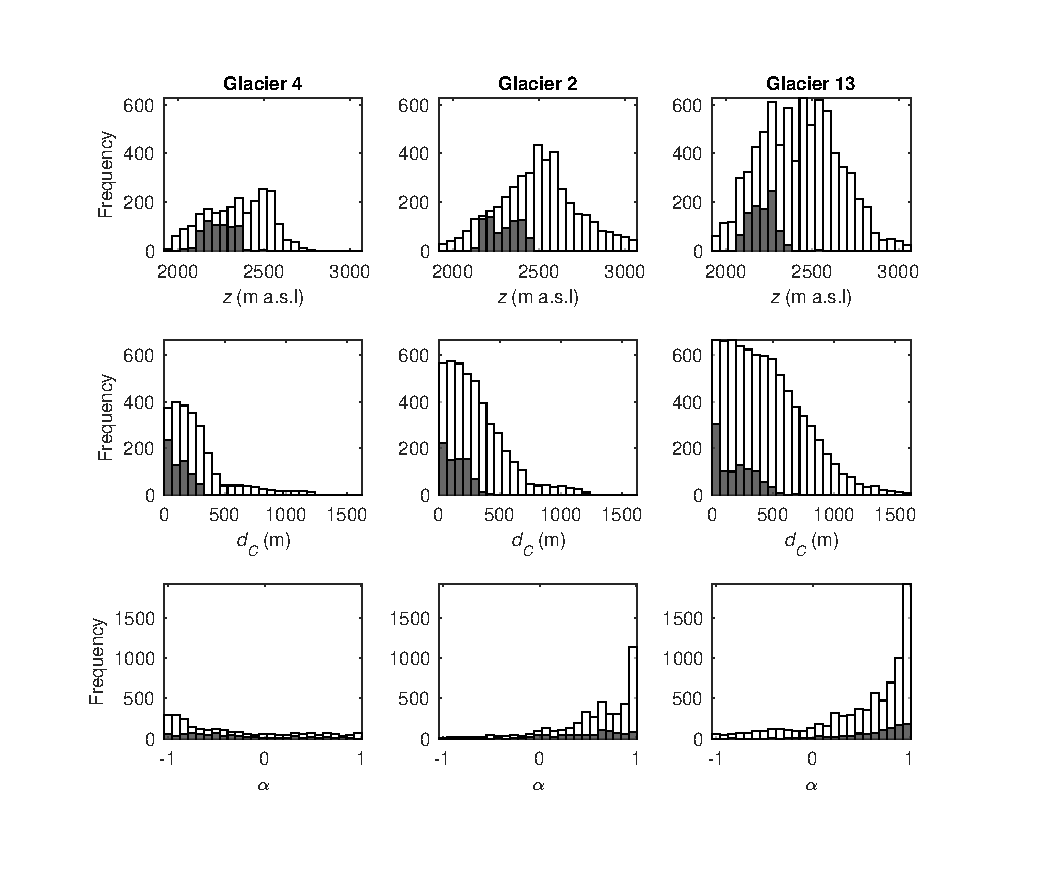
\includegraphics[width =0.9\textwidth]{TopoParamsSampled1.pdf}\\
	\caption{Distribution of sampled (gray bars) and all (white bars) topographic parameters for over Glacier 4 (left column), Glacier 2 (middle column) and Glacier 13 (right column). From top to bottom, topographic parameters are elevation ($z$), distance from centreline ($d_C$), aspect ($\alpha$), slope ($m$), northness ($N$), mean curvature ($\kappa$), and wind redistribution ($Sx$).}
	\label{fig:TopoParamsSampled1}
\end{figure*}

\renewcommand{\thefigure}{S\arabic{figure} (Cont.)}
\addtocounter{figure}{-1}

\begin{figure*}[]
\centering
	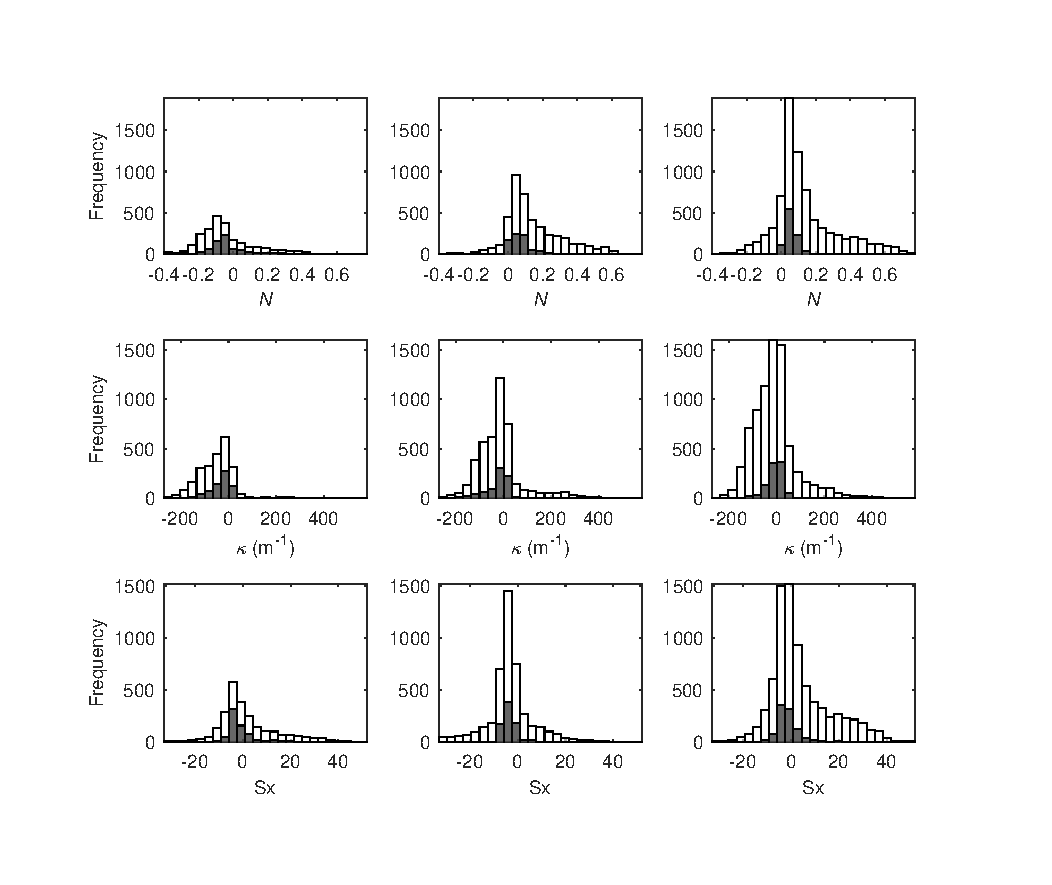
\includegraphics[width =0.9\textwidth]{TopoParamsSampled2.pdf}\\
	\caption{Distribution of sampled (gray bars) and all (white bars) topographic parameters for over Glacier 4 (left column), Glacier 2 (middle column) and Glacier 13 (right column). From top to bottom, topographic parameters are elevation ($z$), distance from centreline ($d_C$), aspect ($\alpha$), slope ($m$), northness ($N$), mean curvature ($\kappa$), and wind redistribution ($Sx$).}
	\label{fig:TopoParamsSampled2}
\end{figure*}


%% TOPO PARAMS TABLE
\begin{landscape}
\begin{table*}[H]
\begin{threeparttable}
   %\captionsetup{singlelinechec\FloatBarrierk=off, skip=4pt}
\caption{Description of topographic parameters used in the linear regression.}
\label{tab:TopoParams}
\begin{tabularx}{24cm}{XXXXX}

\midrule
\textbf{\begin{tabular}[c]{@{}l@{}}Topographic\\ parameter\end{tabular}} & \textbf{Definition} & \textbf{\begin{tabular}[c]{@{}l@{}}Calculation \\ method\end{tabular}} & \textbf{Notes} & \textbf{Source} \\ \midrule
\textbf{Elevation ($z$)} & Height above sea level & Values taken directly from DEM &  &  \\ \midrule
\textbf{Distance from centreline ($d_C$)} & Linear distance from user-defined glacier centreline & Minimum distance between the Easting and Northing of the northwest corner of each grid cell and a manually defined centreline &  &  \\ \midrule
\textbf{Slope ($m$)} & Angle between a plane tangential to the surface (gradient) and the horizontal & \texttt{r.slope.aspect} module in GRASS GIS software run through QGIS &  & \cite{Mitavsova1993, Hofierka2009, Olaya2009} \\ \midrule
\textbf{Aspect ($\alpha$)} & Dip direction of the slope & \texttt{r.slope.aspect} module in GRASS GIS software run through QGIS & $\sin(\alpha)$, a linear quantity describing a slope as north/south facing, is used in the regression & \cite{Mitavsova1993, Hofierka2009, Olaya2009} \\ \midrule
\textbf{Mean curvature ($\kappa$)} & Average of profile (direction of the surface gradient) and tangential (direction of the contour tangent) curvature & \texttt{r.slope.aspect} module in GRASS GIS software run through QGIS & ($+$) mean-concave terrain and ($-$) mean-convex terrain & \cite{Mitavsova1993, Hofierka2009, Olaya2009} \\ \midrule
\textbf{``Northness'' ($N$)} & A value of $-1$ represents a vertical, south facing slope, a value of $+1$ represents a vertical, north facing slope, and a flat surface yields 0 & Product of the cosine of aspect and sine of slope &  & \citep{Molotch2005} \\ \midrule
\textbf{Wind exposure/shelter parameter (Sx)} & Proxy for snow deposition due to wind redistribution & Executable obtained from Adam Winstral that follows the procedure outlined in \cite{Winstral2002} & Calculation based on selecting a cell within a certain angle and distance from the cell of interest that has the greatest upward slope relative to the cell of interest & \citep{Winstral2002}
\end{tabularx}
\end{threeparttable}
\end{table*}
\end{landscape}


\clearpage


\subsection*{Additional results}

%% DENSITY VALUES USED
\begin{table*}[h]
\centering
\caption{Snow density values used for density assignment methods. Density values derived from snow pit (SP) densities and Federal Sampler (FS) densities. Four interpolation methods are chosen: (1) using a mean snow density for all three glaciers (S1 or F1), (2) using a mean density for each glacier (S2 or F2), (3) using a regression between density and elevation (S3 or F3), and (4) inverse-distance weighted mean density (not shown, S4 or F4). Standard deviation (STD) is given for S1/F1 and S2/F2 values and R$^2$ values are given for density--elevation regressions (S3/F3).}
\label{tab:Density}
\begin{tabular}{cccccc}
\midrule
\textbf{} &  & \multicolumn{2}{c}{\textbf{\begin{tabular}[c]{@{}c@{}}SP-derived\\ density (kg\,m$^{-3}$)\end{tabular}}} & \multicolumn{2}{c}{\textbf{\begin{tabular}[c]{@{}c@{}}FS-derived\\ density (kg\,m$^{-3}$)\end{tabular}}} \\
\textbf{} &  & \textit{Mean} & \textit{STD or R$^2$} & \textit{Mean} & \textit{STD or R$^2$} \\ \midrule
\textbf{S1 or F1} &  & 342 & 26 & 318 & 42 \\ \midrule
\multirow{3}{*}{\textbf{S2 or F2}} & G4 & 348 & 13 & 355 & 18 \\
 & G2 & 333 & 26 & 286 & 34 \\
 & G13 & 349 & 38 & 316 & 41 \\ \midrule
\multirow{3}{*}{\textbf{S3 or F3}} & G4 & $0.03z+274$ & 0.16 & $-0.16z+714$ & 0.53 \\
 & G2 & $-0.14z+659$ & 0.75 & $0.24z-282$ & 0.72 \\
 & G13 & $-0.20z+802$ & $>$0.99 & $0.12z+33$ & 0.21
\end{tabular}
\end{table*}



%% RANGE AND NUGGET VALUES
\begin{table}[h]
\centering
\caption{Range and nugget values for simple kriging interpolation}
\label{tab:range&nugget}
\begin{tabular}{ccc}
\midrule
 & \textbf{\begin{tabular}[c]{@{}c@{}}Range \\ (m)\end{tabular}} & \textbf{\begin{tabular}[c]{@{}c@{}}Nugget \\ ($\times10^3$m w.e.)\end{tabular}} \\ \midrule
\textbf{Glacier 4} & 90 & 10.5 \\
\textbf{Glacier 2} & 404 & 3.6 \\
\textbf{Glacier 13} & 444 & 4.8
\end{tabular}
\end{table}

\clearpage

%----------------------------------------------------------------------------------------
%	REFERENCE LIST
%----------------------------------------------------------------------------------------
%
\bibliography{/home/glaciology1/Documents/MastersDocuments/MastersLit}
%\bibliography{/Users/Alexandra/Documents/SFU/MastersDocuments/MastersLit}
\bibliographystyle{igs}

%----------------------------------------------------------------------------------------


\end{document}